%%%%%%%%%%%%%%%%%%%%%%%%%%%%%%%%%%%%%%%%%
% University of Milano Bicocca
% Created by Davide Costantini, Gianlorenzo Martini, Khalil Mohamed Khalil, Lorenzo Occhipinti, Luca Milazzo
% LaTeX Template for simple report
%%%%%%%%%%%%%%%%%%%%%%%%%%%%%%%%%%%%%%%%%

%----------------------------------------------------------------------------------------
%	PACKAGES AND DOCUMENT CONFIGURATIONS
%----------------------------------------------------------------------------------------

\documentclass[12pt]{article} 

\usepackage[left=3cm, right=3cm]{geometry} % insert here document layout options
\usepackage{natbib} % Required to change bibliography style to APA 
\usepackage{tabularx,booktabs,tabulary,array,graphicx,url}
\usepackage{graphicx}
\graphicspath{ {./images/} }
\usepackage[table,xcdraw]{xcolor}
\usepackage{multirow}
\usepackage{caption}
\usepackage[export]{adjustbox}
\usepackage{float}
\usepackage{indentfirst} 
\usepackage{subfig}
\usepackage{listings}
\renewcommand{\figurename}{Fig.}
\usepackage{adjustbox}
\usepackage{pifont}
\usepackage{hyperref} % \usepackage[hidelinks]{hyperref} use the 'hidelinks' option to remove red boxes from links
\newcommand*\rot{\rotatebox{90}} % custom command to rotate columns/rows names in tables


%\usepackage{times} % Uncomment to use the Times New Roman font

%----------------------------------------------------------------------------------------
%	DOCUMENT INFORMATION
%----------------------------------------------------------------------------------------

\title{ Progetto Questionari 1 - Ingegneria del Software  UNIMIB 2021/2022} % Title

\author{Davide Costantini, Gianlorenzo Martini, Khalil Mohamed Khalil, \\ Lorenzo Occhipinti, Luca Milazzo} % Author name

\date{30/01/2022} % Date for the report

\begin{document}

\maketitle % Insert the title, author and date

\newpage
\tableofcontents \newpage
\section{Visione sintetica}

Si chiede di progettare un applicazione Web in grado di gestire questionari su vari argomenti.
Le funzionalit\`{a} richieste sono:
\begin{itemize}
\item Creazione di domande (testuali oppure contenenti immagini) con vari tipi di risposta (e.g., aperta con un minimo e massimo di caratteri, chiusa con scelte multiple);
\item Salvataggio delle domande in un database;
\item Categorizzazione delle domande nel database (e.g., riguardanti un certo argomento);
\item Ricerca e visualizzazione delle domande presenti nel database;
\item Creazione di un questionario partendo da domande gi\`{a} create;
\item Salvataggio dei questionari nel database;
\item Scelta, modifica e cancellazione delle domande e dei questionari;
\item Creazione di un'interfaccia grafica Web per la presentazione dei questionari agli utenti;
\item Compilazione dei questionari da parte degli utenti, che permette il salvataggio temporaneo intermedio e il salvataggio finale a questionario completato;
\item Salvataggio dei questionari compilati nel database;
\item Generazione automatica di un pdf dei questionari completati e notifica via email dell'avvenuta
compilazione e completamento;
\item Ricerca di un questionario nel database (in base a un codice, a una parola presente nel questionario, ecc);
\item Visualizzazione di un questionario presente nel database;
\item Modifica e cancellazione di un questionario nel database;
\item L'applicazione Web deve permettere la compilazione dei questionari a tutti gli utenti;
\item L'applicazione da la possibilit\`{a} agli utenti di registrarsi. Gli utenti registrati possono consultare i questionari che hanno compilato;
\item Per gli utenti non registrati, il sistema fornisce un codice univoco per ogni questionario compilato che pu\`{o} essere usato per visualizzare, modificare e cancellare il questionario compilato.
\end{itemize}

\section{Analisi e progettazione}
\subsection{Glossario}

\begin{table}[H]
\begin{adjustbox}{max width=1.1\textwidth,center}
\begingroup
\setlength{\tabcolsep}{10pt} 
\renewcommand{\arraystretch}{2}
\begin{tabular}{llll}
\multicolumn{3}{c}{\textbf{Glossario}}                                                                                                                                                                                                                                                                                                                                     \\ \hline
\rowcolor[HTML]{3531FF} 
\multicolumn{1}{|l|}{\cellcolor[HTML]{3531FF}{\color[HTML]{FFFFFF} \textbf{ID}}} & \multicolumn{1}{l|}{\cellcolor[HTML]{3531FF}{\color[HTML]{FFFFFF} \textbf{Termine}}} & \multicolumn{1}{l|}{\cellcolor[HTML]{3531FF}{\color[HTML]{FFFFFF} \textbf{Definizione}}}                                                                                                         \\ \hline
\multicolumn{1}{|l|}{1}                                                          & \multicolumn{1}{l|}{Utente}                                                          & \multicolumn{1}{l|}{Un qualsiasi utente che utilizza il sistema.}                                                                                                                                \\ \hline
\multicolumn{1}{|l|}{2}                                                          & \multicolumn{1}{l|}{Utente registrato}                                               & \multicolumn{1}{l|}{Un utente che possiede un account.}                                                                                                                                          \\ \hline
\multicolumn{1}{|l|}{3}                                                          & \multicolumn{1}{l|}{Utente non registrato}                                           & \multicolumn{1}{l|}{Un utente che non possiede un account.}                                                                                                                                      \\ \hline
\multicolumn{1}{|l|}{4}                                                          & \multicolumn{1}{l|}{Servizio email}                                                  & \multicolumn{1}{l|}{Il sottosistema che permette l'effettivo invio di email.}                                                                                                                    \\ \hline
\multicolumn{1}{|l|}{5}                                                          & \multicolumn{1}{l|}{Domanda}                                                         & \multicolumn{1}{l|}{Un elemento testuale o multimediale (immagine) contenente delle risposte.}                                                                                                   \\ \hline
\multicolumn{1}{|l|}{6}                                                          & \multicolumn{1}{l|}{Riposta}                                                         & \multicolumn{1}{l|}{\begin{tabular}[c]{@{}l@{}}Associata ad una domanda può essere:\\ - Aperta con eventuale numero massimo e/o minimo di caratteri\\ - Chiuse con scelte multiple\end{tabular}} \\ \hline
\multicolumn{1}{|l|}{7}                                                          & \multicolumn{1}{l|}{Questionario}                                                    & \multicolumn{1}{l|}{minimo e massimo di caratteri, chiusa con scelte multiple}                                                                                                                   \\ \hline
\end{tabular}
\endgroup
\end{adjustbox}
\end{table}


\subsection{Casi d'uso}
In questa sezione sono presentati gli attori del sistema ed i relativi casi d'uso. Per alcuni di essi sono riportate anche le loro descrizioni dettagliate.

\begin{table}[htbp]
\centering
\begin{tabular}{lll}
\multicolumn{3}{c}{\textbf{{\large Attori del sistema}}}                                                                                                                                                                                                          \\ \hline
\rowcolor[HTML]{3531FF} 
\multicolumn{1}{|l|}{\cellcolor[HTML]{3531FF}{\color[HTML]{FFFFFF} \textbf{ID}}} & \multicolumn{1}{l|}{\cellcolor[HTML]{3531FF}{\color[HTML]{FFFFFF} \textbf{Nome}}} & \multicolumn{1}{l|}{\cellcolor[HTML]{3531FF}{\color[HTML]{FFFFFF} \textbf{Tipo}}} \\ \hline                                                   
\multicolumn{1}{|l|}{1}                                                          & \multicolumn{1}{l|}{Utente registrato}                                            & \multicolumn{1}{l|}{Primario}             

										\\ \hline
\multicolumn{1}{|l|}{2}                                                          & \multicolumn{1}{l|}{Utente non registrato}                                        & \multicolumn{1}{l|}{Primario}                                                     \\ \hline
\multicolumn{1}{|l|}{3}                                                          & \multicolumn{1}{l|}{Servizio email}                                        & \multicolumn{1}{l|}{Di Supporto}   
										\\ \hline
\end{tabular}
\end{table}


\begin{table}[H]
\begin{adjustbox}{max width=1.1\textwidth,center}
\begingroup
\setlength{\tabcolsep}{10pt} 
\renewcommand{\arraystretch}{2}
\begin{tabular}{llll}
\multicolumn{4}{c}{\textbf{{\LARGE Casi d'uso - Formato breve}}}                                                                                                                                                                                                                                                                                                                                                                                                                                                            \\ \hline
\rowcolor[HTML]{3531FF} 
\multicolumn{1}{|l|}{\cellcolor[HTML]{3531FF}{\color[HTML]{FFFFFF} \textbf{ID}}} & \multicolumn{1}{l|}{\cellcolor[HTML]{3531FF}{\color[HTML]{FFFFFF} \textbf{Nome}}}                             & \multicolumn{1}{l|}{\cellcolor[HTML]{3531FF}{\color[HTML]{FFFFFF} \textbf{Attore}}}                    & \multicolumn{1}{l|}{\cellcolor[HTML]{3531FF}{\color[HTML]{FFFFFF} \textbf{Descrizione}}}                                                                                                               \\ \hline
\multicolumn{1}{|l|}{1}                                                          & \multicolumn{1}{l|}{Effettua Login}                                                                           & \multicolumn{1}{l|}{Utente registrato}                                                                 & \multicolumn{1}{l|}{\begin{tabular}[c]{@{}l@{}}L'utente, dopo aver inserito le sue credenziali verificate dal sistema, \\ effettua l'accesso all'applicazione.\end{tabular}}                           \\ \hline
\multicolumn{1}{|l|}{2}                                                          & \multicolumn{1}{l|}{Effettua Logout}                                                                          & \multicolumn{1}{l|}{Utente registrato}                                                                 & \multicolumn{1}{l|}{L'utente registrato effettua il logout dal sistema.}                                                                                                                               \\ \hline
\multicolumn{1}{|l|}{3}                                                          & \multicolumn{1}{l|}{Creazione domanda}                                                                        & \multicolumn{1}{l|}{Utente registrato}                                                                 & \multicolumn{1}{l|}{\begin{tabular}[c]{@{}l@{}}L'utente registrato crea domande, testuali o contenenti immagini,\\  con risposte chiuse o aperte ed il sistema le memorizza .\end{tabular}}            \\ \hline
\multicolumn{1}{|l|}{4}                                                          & \multicolumn{1}{l|}{Ricerca domanda}                                                                          & \multicolumn{1}{l|}{Utente registrato}                                                                 & \multicolumn{1}{l|}{L'utente cerca le domande presenti nel sistema e le visualizza.}                                                                                                                   \\ \hline
\multicolumn{1}{|l|}{5}                                                          & \multicolumn{1}{l|}{Creazione questionario}                                                                   & \multicolumn{1}{l|}{Utente registrato}                                                                 & \multicolumn{1}{l|}{\begin{tabular}[c]{@{}l@{}}L'utente registrato crea un questionario, poi memorizzato dal sistema, \\ partendo da domande gi\`{a} create.\end{tabular}}                                 \\ \hline
\multicolumn{1}{|l|}{6}                                                          & \multicolumn{1}{l|}{Modifica domanda}                                                                         & \multicolumn{1}{l|}{Utente registrato}                                                                 & \multicolumn{1}{l|}{L'utente registrato modifica una domanda che ha creato.}                                                                                                                           \\ \hline
\multicolumn{1}{|l|}{7}                                                          & \multicolumn{1}{l|}{Cancellazione domanda}                                                                    & \multicolumn{1}{l|}{Utente registrato}                                                                 & \multicolumn{1}{l|}{L'utente registrato cancella la domanda che ha creato.}                                                                                                                            \\ \hline
\multicolumn{1}{|l|}{8}                                                          & \multicolumn{1}{l|}{Modifica questionario}                                                                    & \multicolumn{1}{l|}{Utente registrato}                                                                 & \multicolumn{1}{l|}{L'utente registrato modifica un questionario che ha creato.}                                                                                                                       \\ \hline
\multicolumn{1}{|l|}{9}                                                          & \multicolumn{1}{l|}{Cancellazione questionario}                                                               & \multicolumn{1}{l|}{Utente registrato}                                                                 & \multicolumn{1}{l|}{L'utente registrato cancella i questionari che ha creato.}                                                                                                                         \\ \hline
\multicolumn{1}{|l|}{10}                                                         & \multicolumn{1}{l|}{Modifica risposta}                                                                        & \multicolumn{1}{l|}{Utente registrato}                                                                 & \multicolumn{1}{l|}{L'utente modifica le sue risposte ai questionari.}                                                                                                                                 \\ \hline
\multicolumn{1}{|l|}{11}                                                         & \multicolumn{1}{l|}{Cancellazione risposta}                                                                   & \multicolumn{1}{l|}{Utente registrato}                                                                 & \multicolumn{1}{l|}{L'utente elimina le sue risposte ai questionari.}                                                                                                                                  \\ \hline
\multicolumn{1}{|l|}{12}                                                         & \multicolumn{1}{l|}{Compilazione questionario}                                                                & \multicolumn{1}{l|}{Utente registrato}                                                                 & \multicolumn{1}{l|}{L'utente compila i questionari inserendo delle risposte.}                                                                                                                          \\ \hline
\multicolumn{1}{|l|}{13}                                                         & \multicolumn{1}{l|}{\begin{tabular}[c]{@{}l@{}}Notifica del completamento \\ di un questionario\end{tabular}} & \multicolumn{1}{l|}{Servizio email}                                                                       & \multicolumn{1}{l|}{\begin{tabular}[c]{@{}l@{}}Il sistema esterno invia una email all'utente in cui lo avvisa del\\ completamento di un questionario con un PDF delle risposte date.\end{tabular}}     \\ \hline
\multicolumn{1}{|l|}{14}                                                         & \multicolumn{1}{l|}{Ricerca di un questionario}                                                               & \multicolumn{1}{l|}{\begin{tabular}[c]{@{}l@{}}Utente registrato\\ Utente non registrato\end{tabular}} & \multicolumn{1}{l|}{\begin{tabular}[c]{@{}l@{}}L'utente può cercare un questionario tra quelli presenti nel sistema \\ in base a un codice, a una parola presente nel questionario, ecc…\end{tabular}} \\ \hline
\multicolumn{1}{|l|}{15}                                                         & \multicolumn{1}{l|}{Effettua registrazione}                                                                   & \multicolumn{1}{l|}{Utente non registrato}                                                             & \multicolumn{1}{l|}{L'utente effettua la registrazione nel sistema.}                                                                                                                                   \\ \hline
\end{tabular}
\endgroup
\end{adjustbox}
\end{table}

\begin{figure}[H]
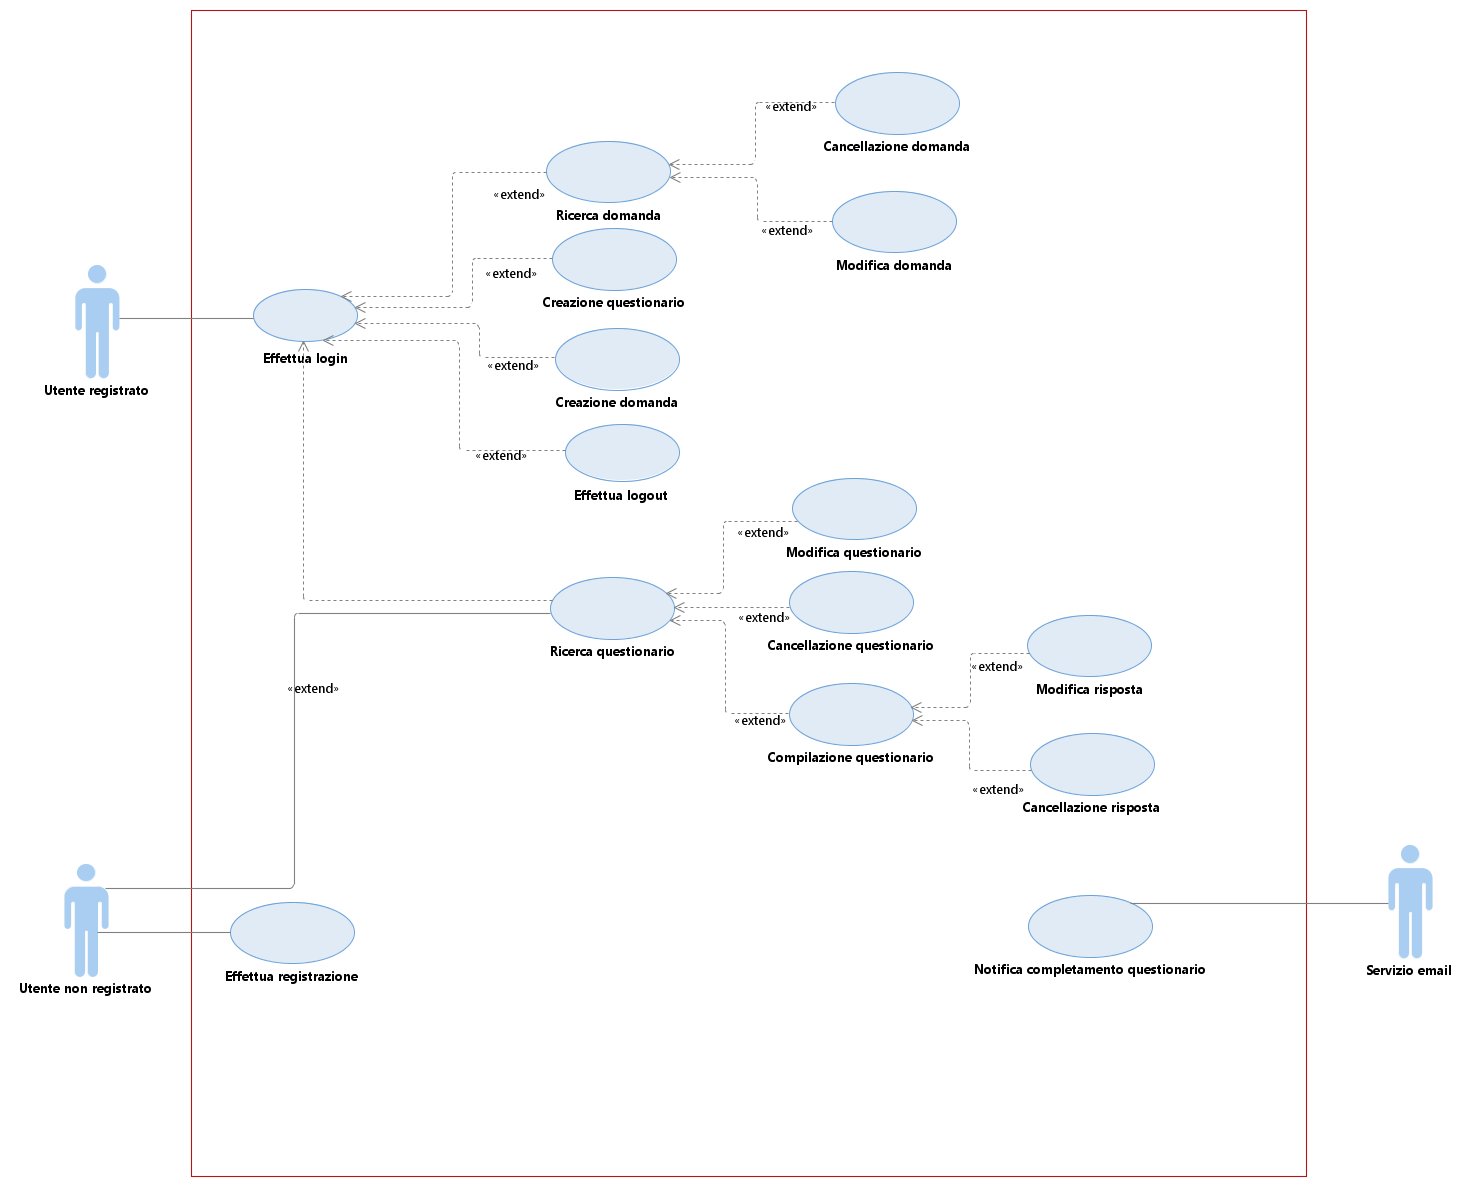
\includegraphics[scale=0.45, left]{fig_usecase_diagram.png}
\caption{Diagramma dei casi d'uso}
\end{figure}

\subsection{Requisiti non funzionali}


\begin{table}[H]
\begin{adjustbox}{max width=1.1\textwidth,center}
\begingroup
\setlength{\tabcolsep}{10pt} 
\renewcommand{\arraystretch}{2}
\begin{tabular}{lllll}     
\multicolumn{5}{c}{\textbf{{\LARGE Tabella dei fattori e promemoria tecnici}}}                                                                                                                                                                                                                                                                                                                                                                         \\ \hline
\rowcolor[HTML]{3531FF} 
\multicolumn{1}{|l|}{\cellcolor[HTML]{3531FF}{\color[HTML]{FFFFFF} \textbf{ID}}} & \multicolumn{1}{l|}{\cellcolor[HTML]{3531FF}{\color[HTML]{FFFFFF} \textbf{Descrizione}}} & \multicolumn{1}{l|}{\cellcolor[HTML]{3531FF}{\color[HTML]{FFFFFF} \textbf{Tipo}}} & \multicolumn{1}{l|}{\cellcolor[HTML]{3531FF}{\color[HTML]{FFFFFF} \textbf{Misura}}} & \multicolumn{1}{l|}{\cellcolor[HTML]{3531FF}{\color[HTML]{FFFFFF} \textbf{Approccio}}} \\ \hline
\multicolumn{1}{|l|}{1}                                                          & \multicolumn{1}{l|}{Il sistema deve essere sempre accessibile.}                          & \multicolumn{1}{l|}{Di prodotto}                                                  & \multicolumn{1}{l|}{Disponibilità}                                                  & \multicolumn{1}{l|}{Istanze multiple}                                                  \\ \hline
\multicolumn{1}{|l|}{2}                                                          & \multicolumn{1}{l|}{Il sistema deve riuscire a gestire molte connessioni contemporanee.} & \multicolumn{1}{l|}{Di prodotto}                                                  & \multicolumn{1}{l|}{Efficienza}                                                     & \multicolumn{1}{l|}{Load balancing}                                                    \\ \hline
\multicolumn{1}{|l|}{3}                                                          & \multicolumn{1}{l|}{Il sistema deve garantire la persistenza dei dati.}                  & \multicolumn{1}{l|}{Di prodotto}                                                  & \multicolumn{1}{l|}{Affidabilità}                                                   & \multicolumn{1}{l|}{Replica sets}                                                      \\ \hline
\multicolumn{1}{|l|}{4}                                                          & \multicolumn{1}{l|}{Il sistema deve garantire la protezione dei dati.}                   & \multicolumn{1}{l|}{Di prodotto}                                                  & \multicolumn{1}{l|}{Sicurezza}                                                      & \multicolumn{1}{l|}{Utilizzo di protocolli di rete sicuri (HTTPS)}                     \\ \hline
\end{tabular}
\endgroup
\end{adjustbox}
\end{table}


\subsection{Design Principles}
Design Principles utilizzati durante la creazione del progetto.
\begin{itemize}
	\item \textbf{Principio di sostituzione di Liskov}: Gli oggetti di un sottotipo di un oggetto possono essere sostituiti dall'oggetto di cui sono sottotipo senza alterare la correttezza del programma.
\end{itemize}

\subsection{SSD}
Qui di seguit sono presenti gli SSD riguardanti i seguenti scenari:
\begin{itemize}
\item Creazione del questionario
\end{itemize}

\begin{figure}[H]
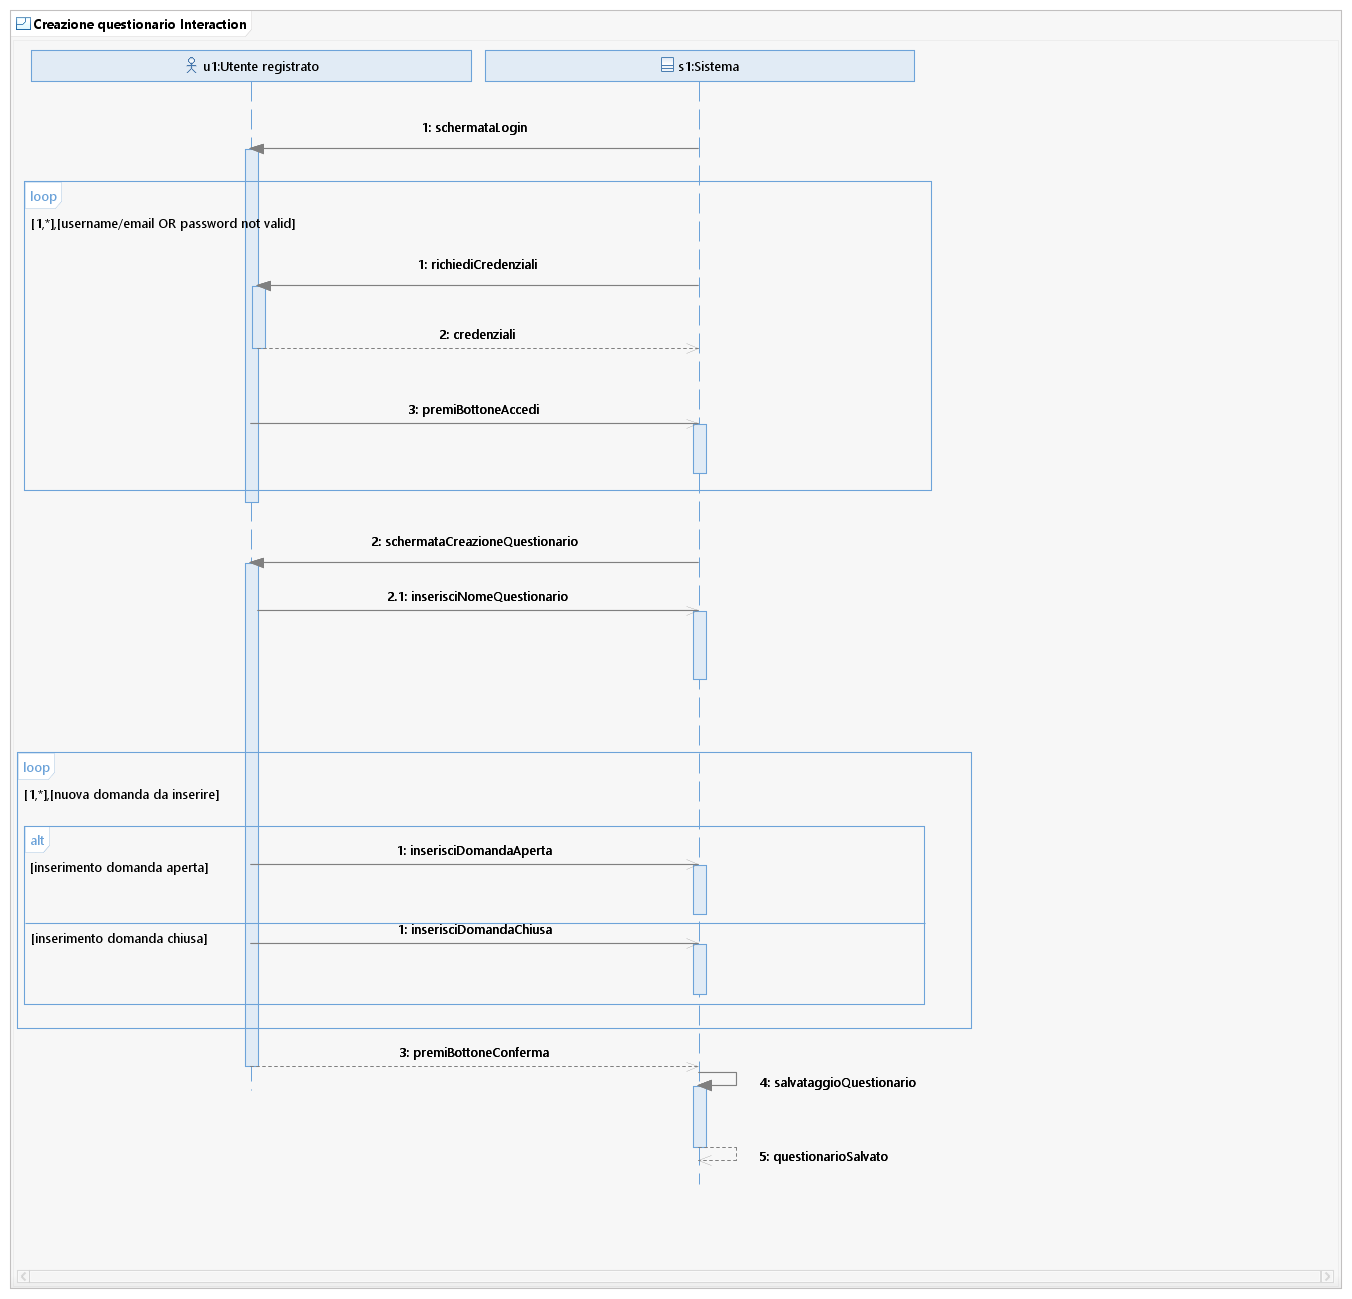
\includegraphics[scale=0.5, left]{UNIMIBModule_CreazionequestionarioSequenceDiagram.png}
\caption{SSD - Creazione del questionario}
\end{figure}



\subsection{Modello di dominio}
\begin{figure}[H]
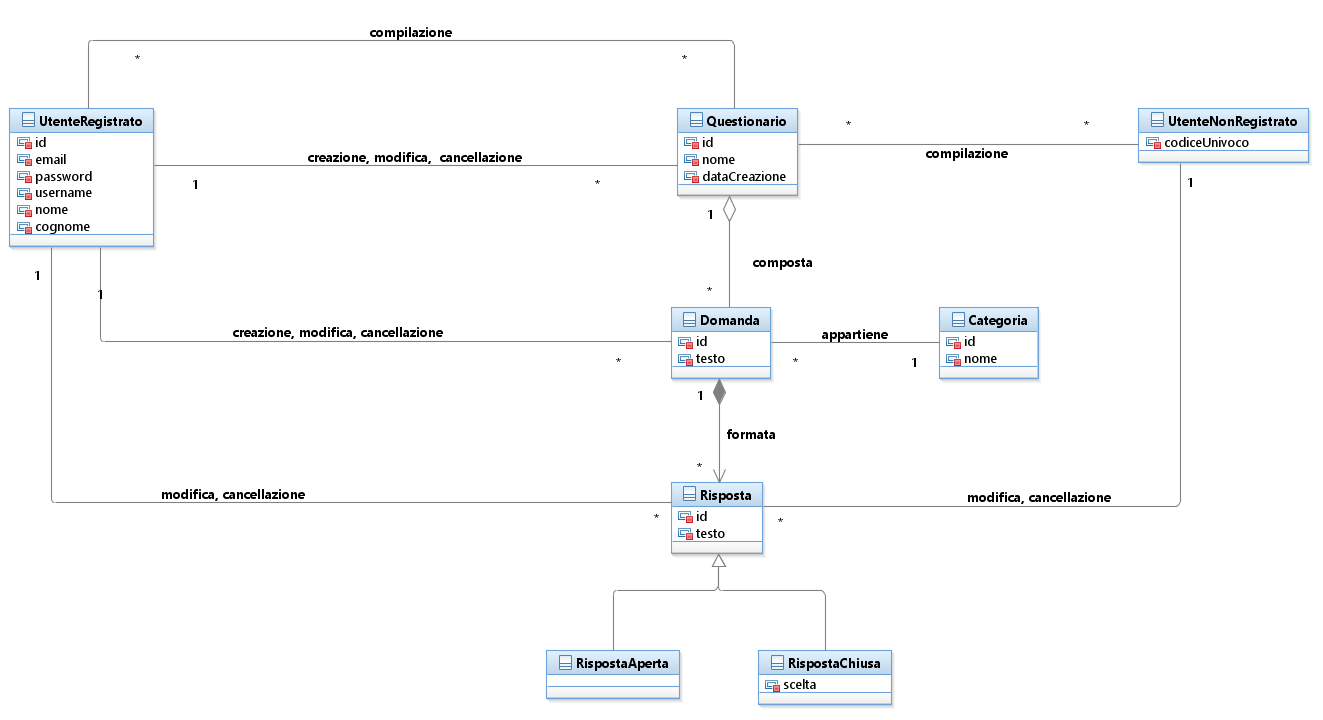
\includegraphics[scale=0.5, left]{UNIMIBModule_UniMiBModuleDomainLayer.png}
\caption{Modello di dominio}
\end{figure}


\subsection{Diagramma delle classi di progettazione}
\subsection{Diagrammi di sequenza}
\subsection{Diagrammi di stato}
\subsection{Diagrammi di attivit\`{a}}
\subsection{Diagramma dell'architettura software}
\subsection{Diagramma di deployment}
\subsection{Modello E-R}
\section{Sviluppo}
\subsection{Piano dello sprint}
\`{E} adottato un metodo di processo di sviluppo Agile seguendo le direttive dell' Unified Process. Il Product backlog contiene i task, normalmente associati ad un caso d'uso,  da sviluppare nei vari sprint. Ogni sprint prevede le seguenti fasi:
\begin{itemize}
\item {\textbf {Sprint meeting}} per la composizione dello sprint backlog;
\item {\textbf {Analisi e progettazione}}  per aggiornare o creare componenti UML utili al task;
\item {\textbf {Bulding e testing}}  per sviluppare il task con la tecnica dell'extreme programming (coppia tester-developer);
\item {\textbf {Review e refactoring}} per la revisione generale del lavoro effettuato e della qualità del codice (architectural smell, code smell ecc...);
\item {\textbf {Retrospective meeting}} per chiudere con il team lo sprint presentando problemi, modifiche ecc...

\end{itemize}

\subsection{Workflow per la Continuos Integration}


%----------------------------------------------------------------------------------------


\end{document}
